



\begin{figure}[t]
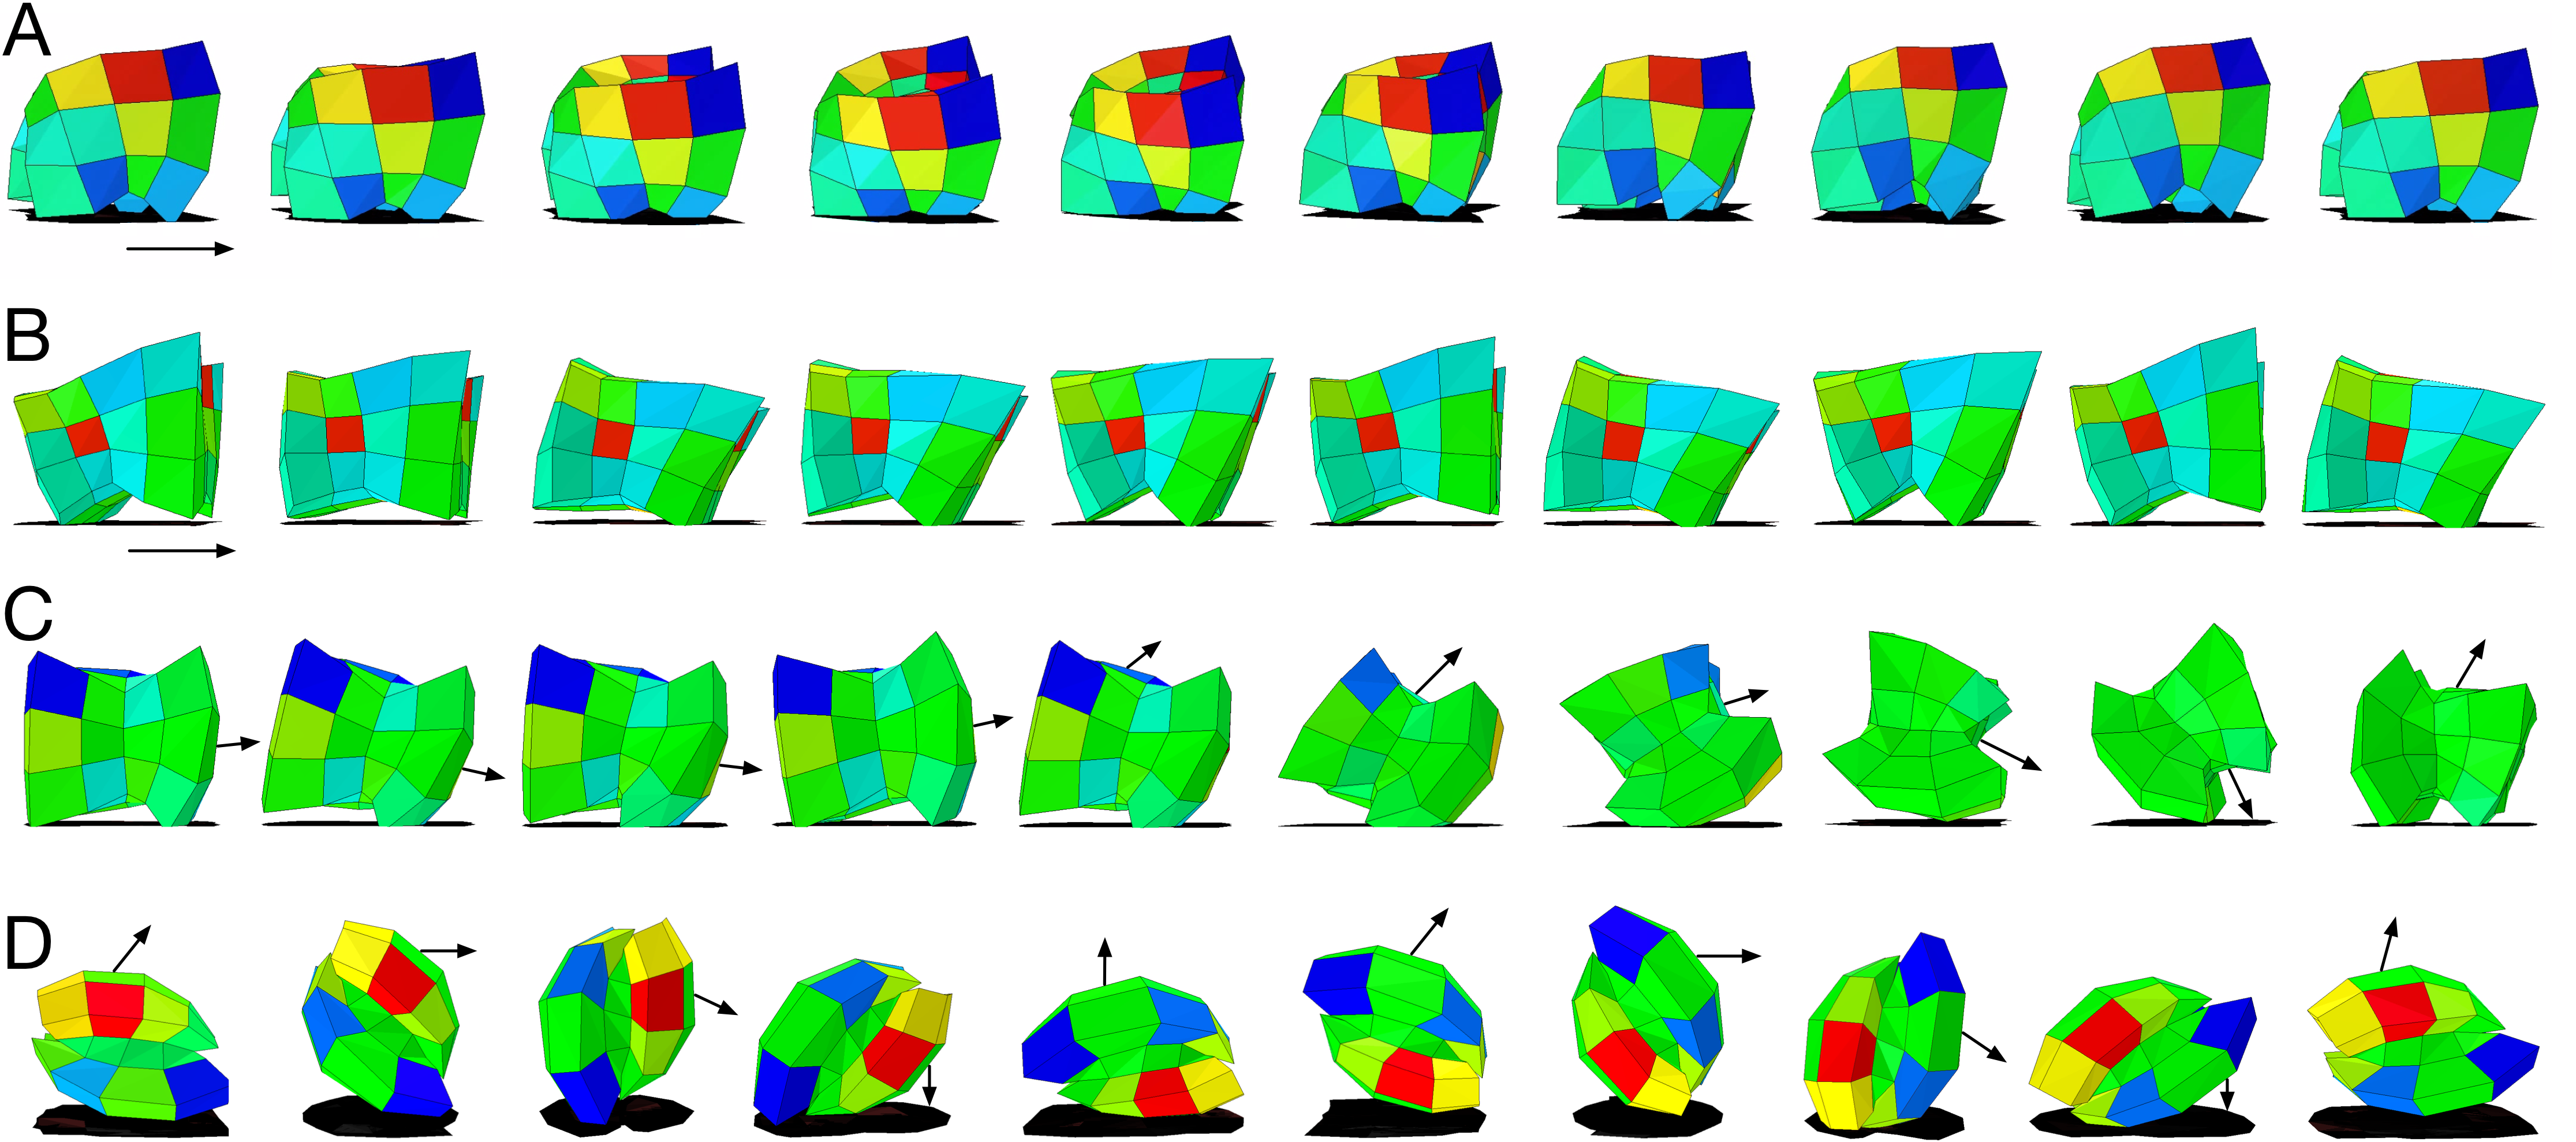
\includegraphics[width=\linewidth]{Chapter04/Fig2}
\caption{\label{fig:trot-gallop-roll}\textbf{Evolved behavior.}
Each row depicts a different evolved robot moving from left to right. 
Voxels in this figure are colored by the amount of subsequent morphological development remaining at that cell: blue indicates shrinking voxels $(\ell_k > \ell_k^*)$, red indicates growing voxels $(\ell_k < \ell_k^*)$, green indicates little to no change either way $(\ell_k \cong \ell_k^*)$.
(A) An evolved trotting soft quadruped with a two-beat gait synchronizing diagonal pairs of legs. 
(B) A galloping adult robot which goes fully airborne mid-gait.
(C) A galloping juvenile robot which develops into a rolling adult form. 
(D) A rolling juvenile robot at 10 points in ontogeny immediately after birth.
Arrows indicate the general directionality of movement,  
but this is more precisely captured by
Supplementary \href{https://youtu.be/Ee2sU-AZWC4}{\color{blue}Video S1}. 
}
\end{figure}


\begin{figure}[t]
\centering
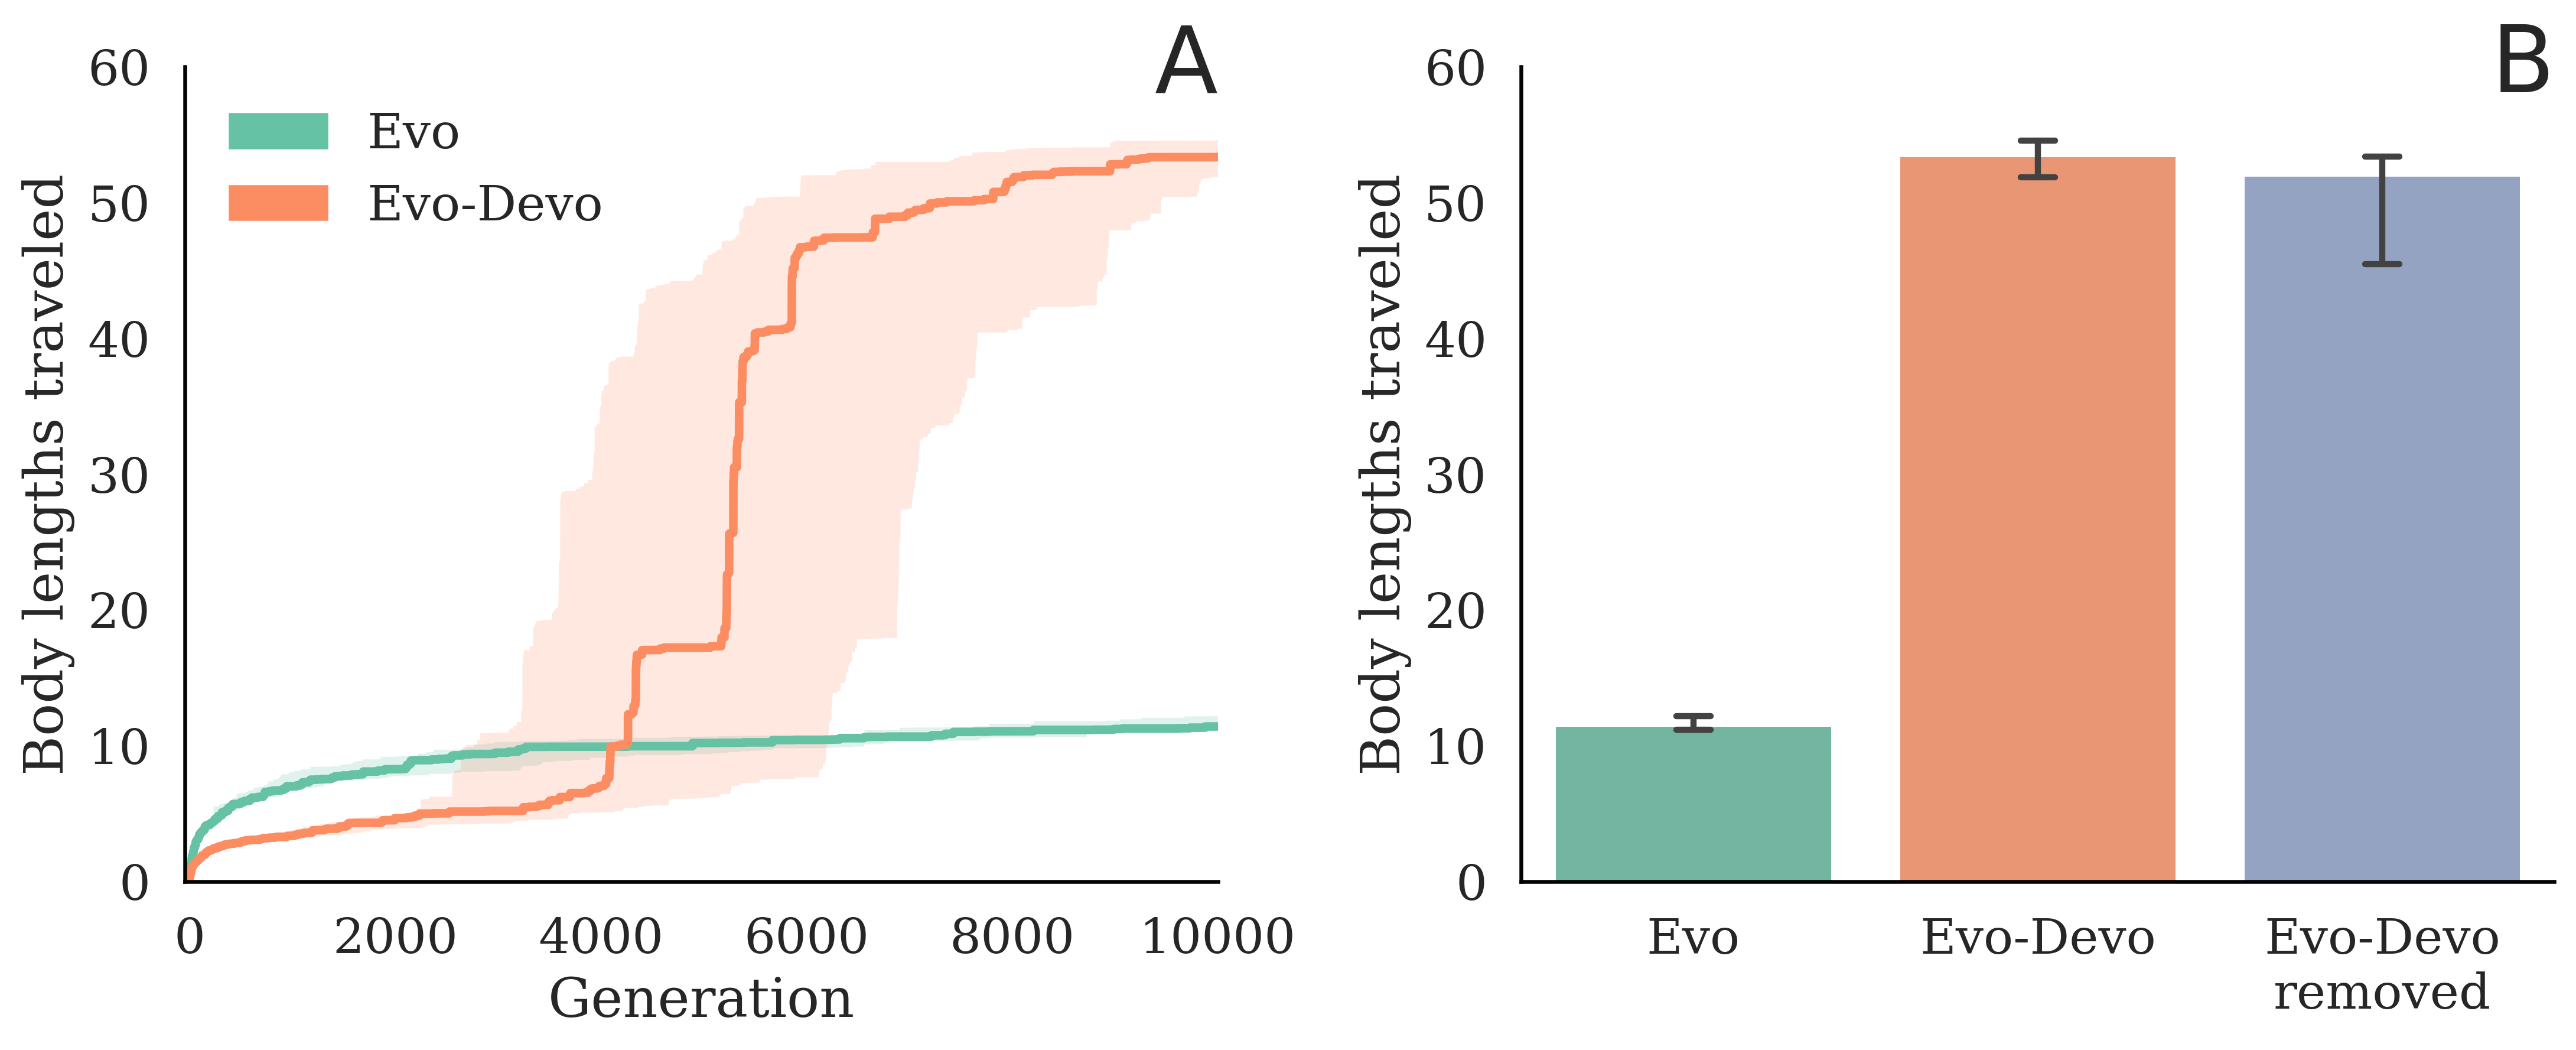
\includegraphics[width=0.9\linewidth]{Chapter04/Fig3}
\caption{\label{fig-fitness}\textbf{Evolvability and development.} Morphological development drastically increases evolvability (A), even when development is manually removed from the evolved systems (the run champions) by setting the final parameter values equal to their starting values ($\ell_k^*=\ell_k$ and $\phi_k^*=\phi_k$), in each voxel (B).
Median fitness is plotted with 95\% bootstrapped confidence intervals for three treatments: evolving but non-developmental robots (Evo), evolving and developing robots (Evo-Devo), and evolving and developing robots evaluated at the end of evolution with their development removed (Evo-Devo removed).
Fitness of just the final, evolved populations (at generation 10000) are plotted in B.}
\end{figure}


\begin{figure}[t]
\centering
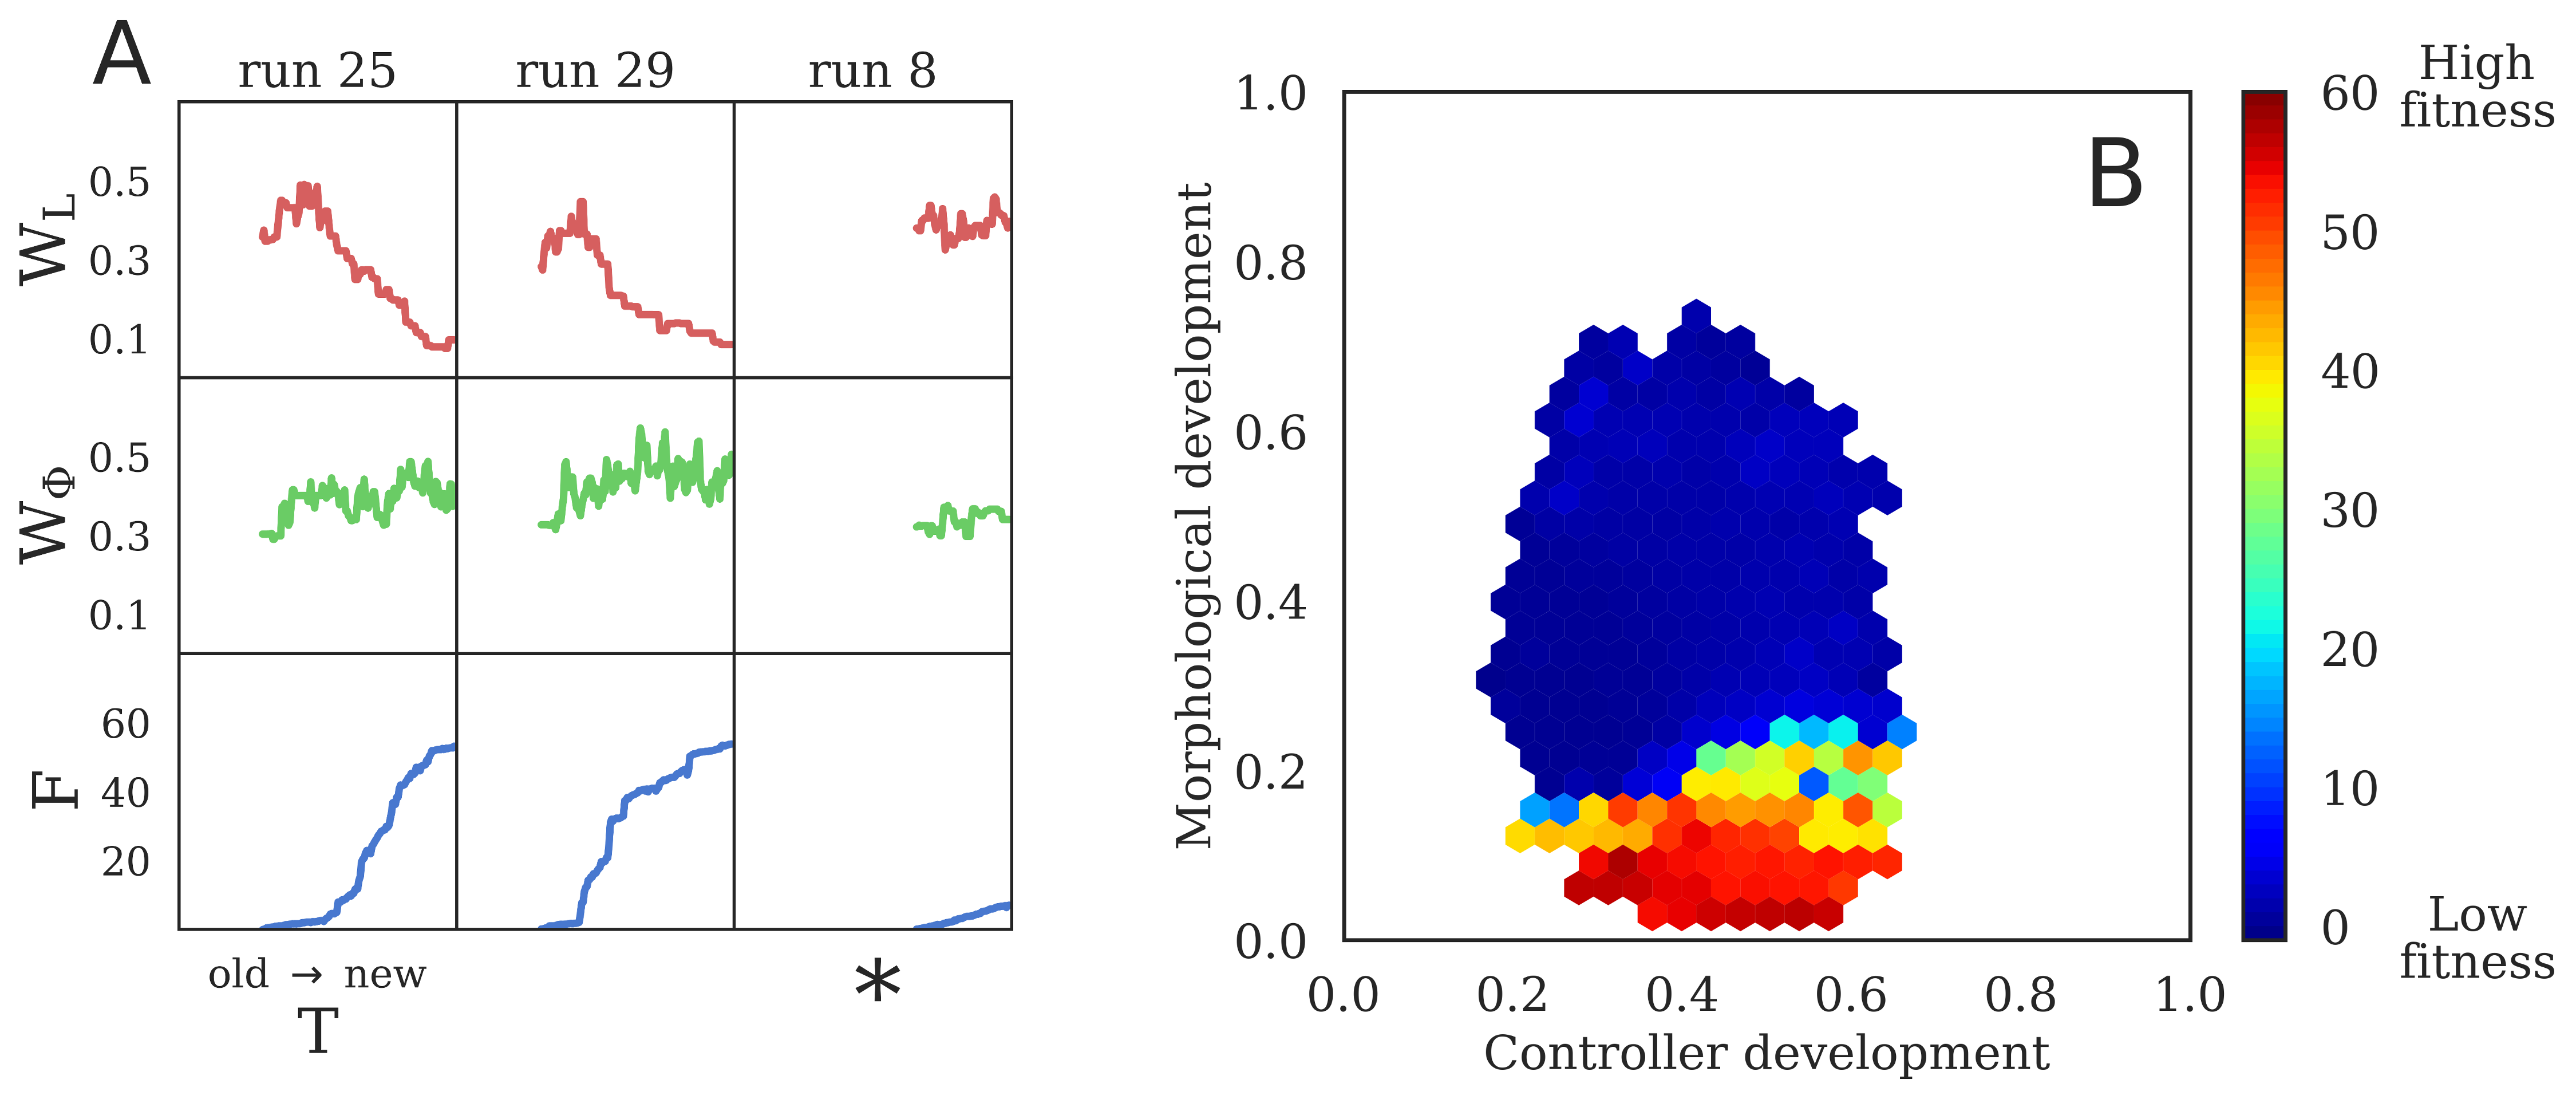
\includegraphics[width=\linewidth]{Chapter04/Fig4}
\caption{\label{fig-correlation}\textbf{Differential canalization.} 
Developmental windows (i.e.~the total lifetime developmental change) for morphology, $W_L$ (see Equation \ref{eq-WL}), and controller, $W_{\Phi}$ (see Equation \ref{eq-WPhi}), alongside fitness $F$.
(A) Three representative lineages taken from Supplementary Fig. \ref{fig:S1}, % S1, 
which displays the lineages of all 30 Evo-Devo run champions. Evolutionary time $T$ moves from the oldest ancestor (left) to the run champion (right). A general trend emerges wherein lineages initially increase their morphological development in $T$ (rising red curves) and subsequently decrease morphological development to almost zero (falling red curves). Five of the 30 evolutionary trials, annotated by {\Large $\ast$}, fell into a local optima.
(B) Median fitness as a function of morphology and controller development windows $(W_L,\; W_{\Phi})$, for all Evo-Devo designs evaluated. 
Overall, the fastest designs tend to have small amounts of morphological development, but are free to explore alternative control policies.}
\end{figure}

\begin{figure}[t]
\centering
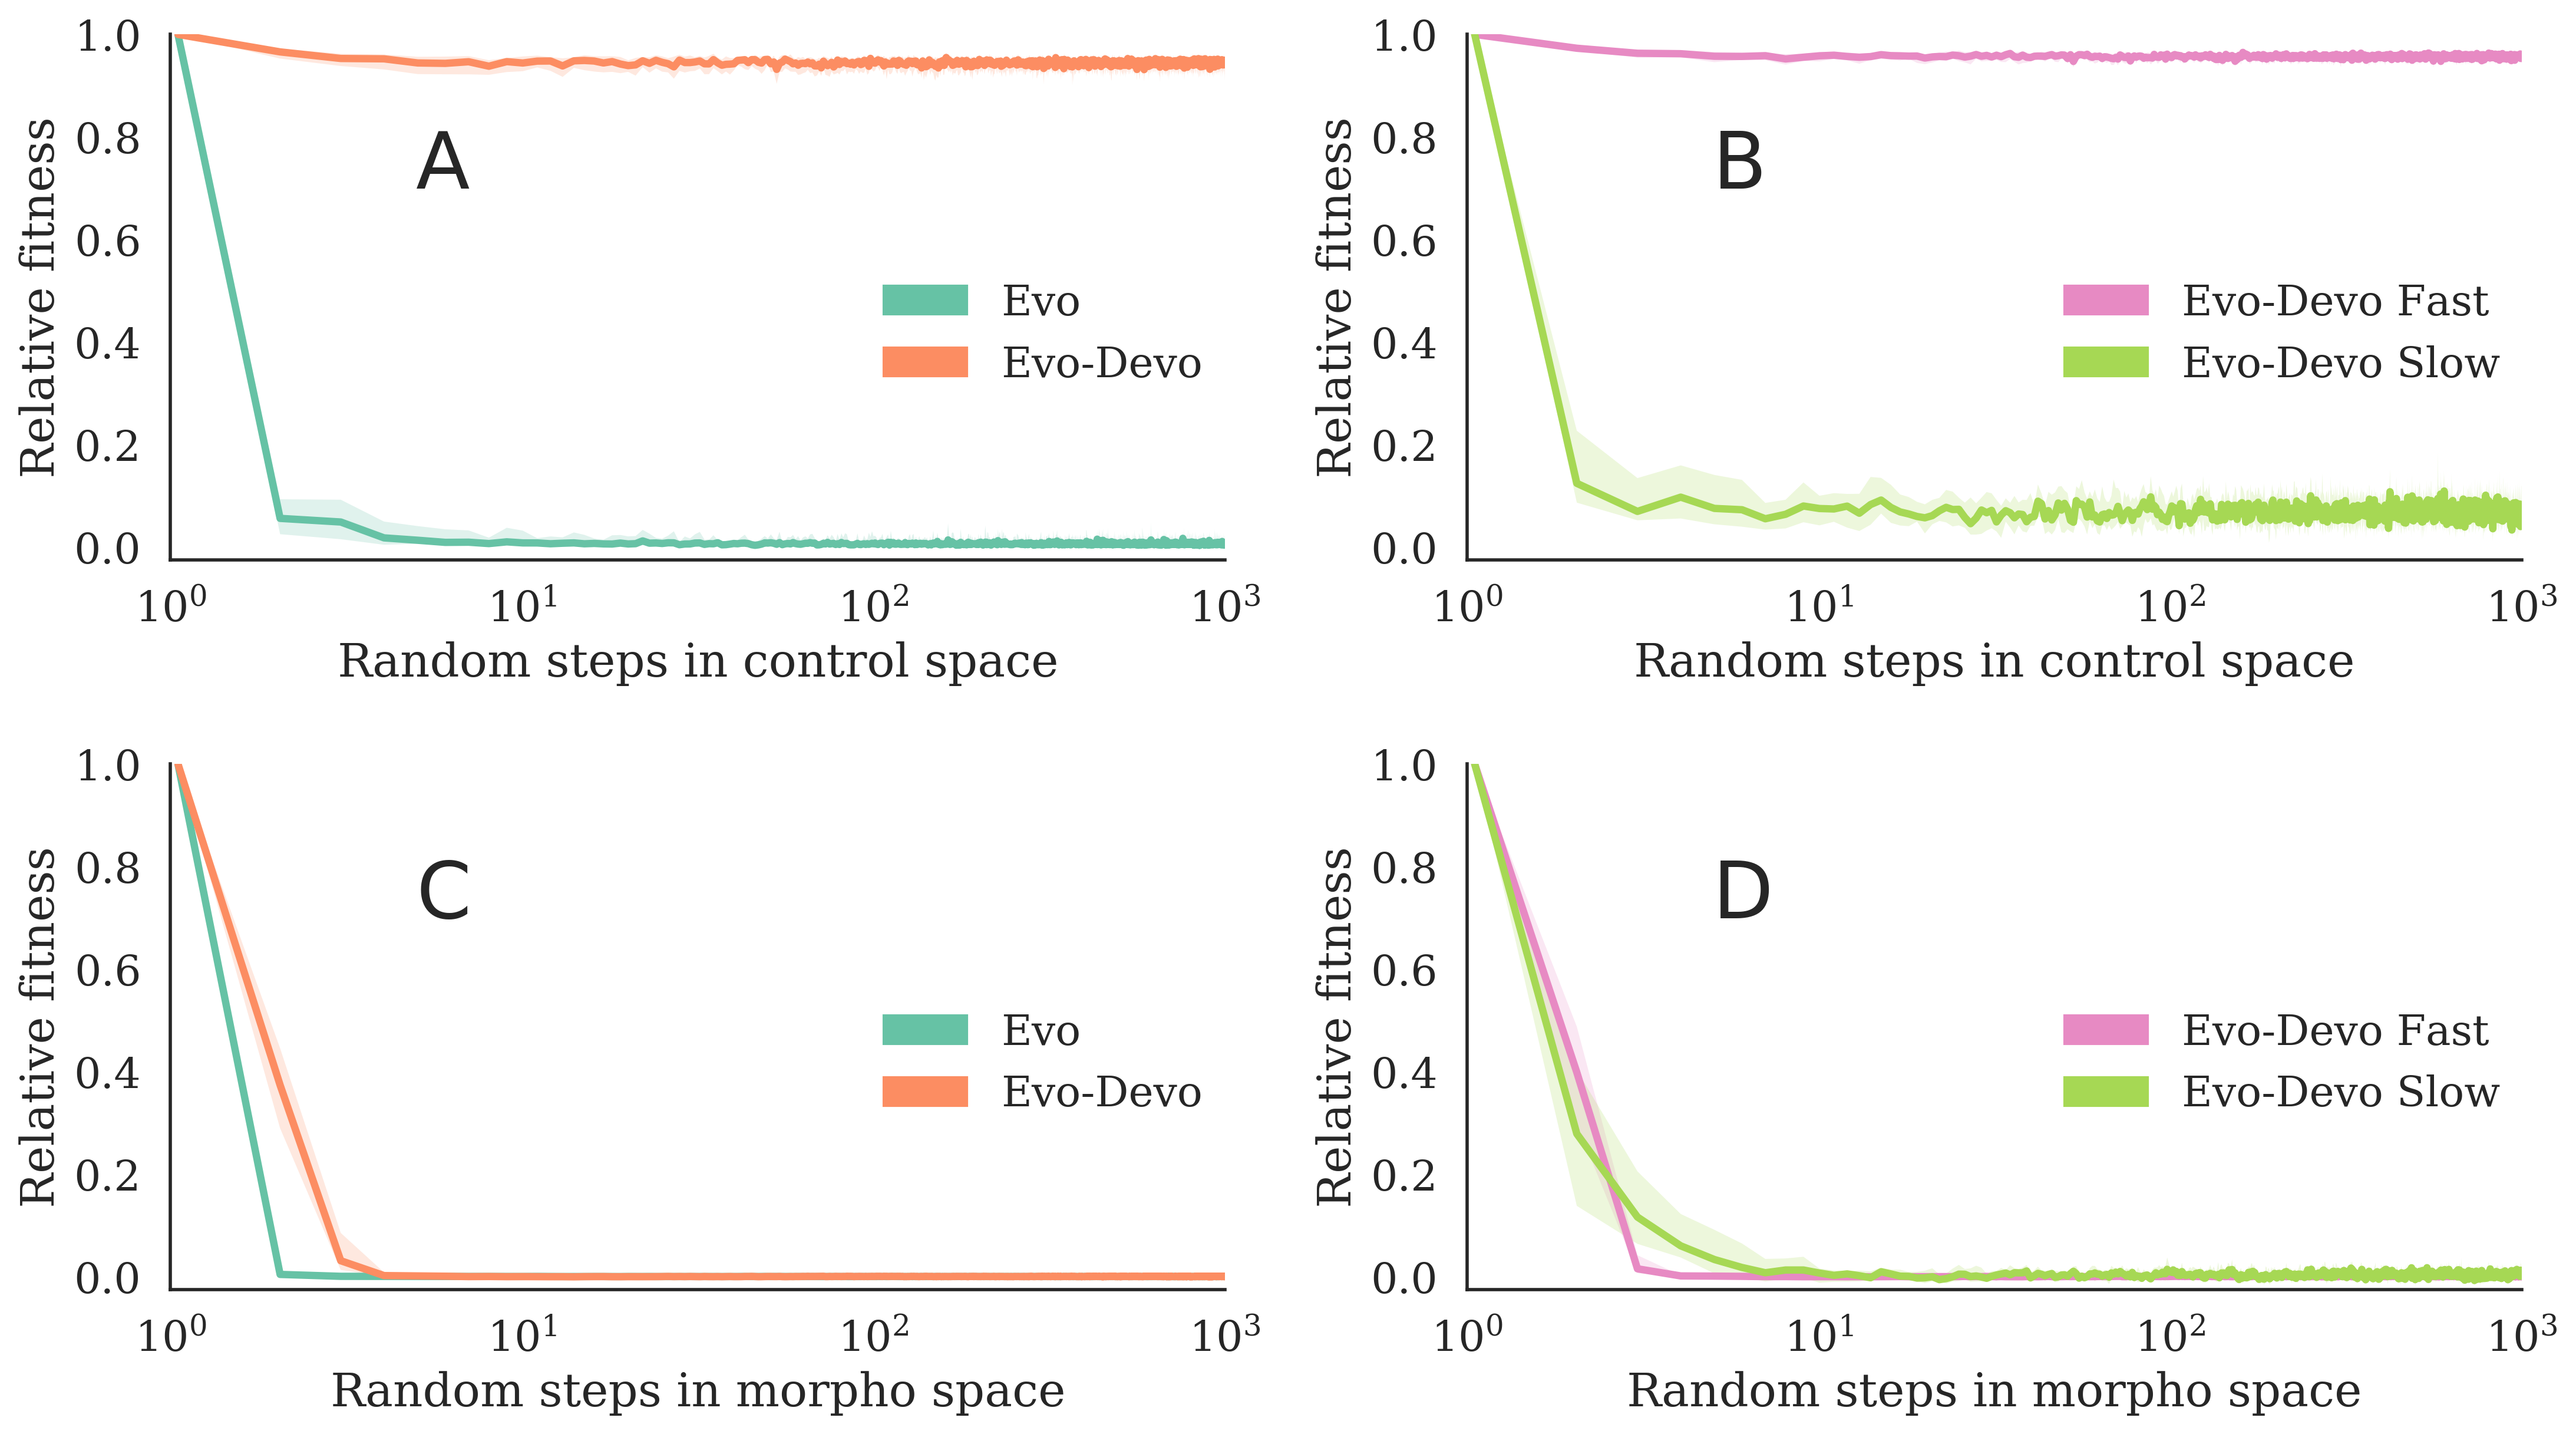
\includegraphics[width=\linewidth]{Chapter04/Fig5}
\caption{\label{fig-random-walks}\textbf{Sensitivity to morphological and control mutations.}
Ten random walks were taken from each run champion.
(A) Successive \textit{control} mutations to the Evo and Evo-Devo run champions.
(B) The previous Evo-Devo results separately for fast and slow design types.
(C) Successive \textit{morphological} mutations to the Evo and Evo-Devo run champions.
(D) The previous Evo-Devo results separately for fast and slow design types. Medians plotted with 99\% confidence intervals.
The faster Evo-Devo robots tend to possess body plans that are robust to control mutations.}
\end{figure}

\begin{figure}[t]
\centering
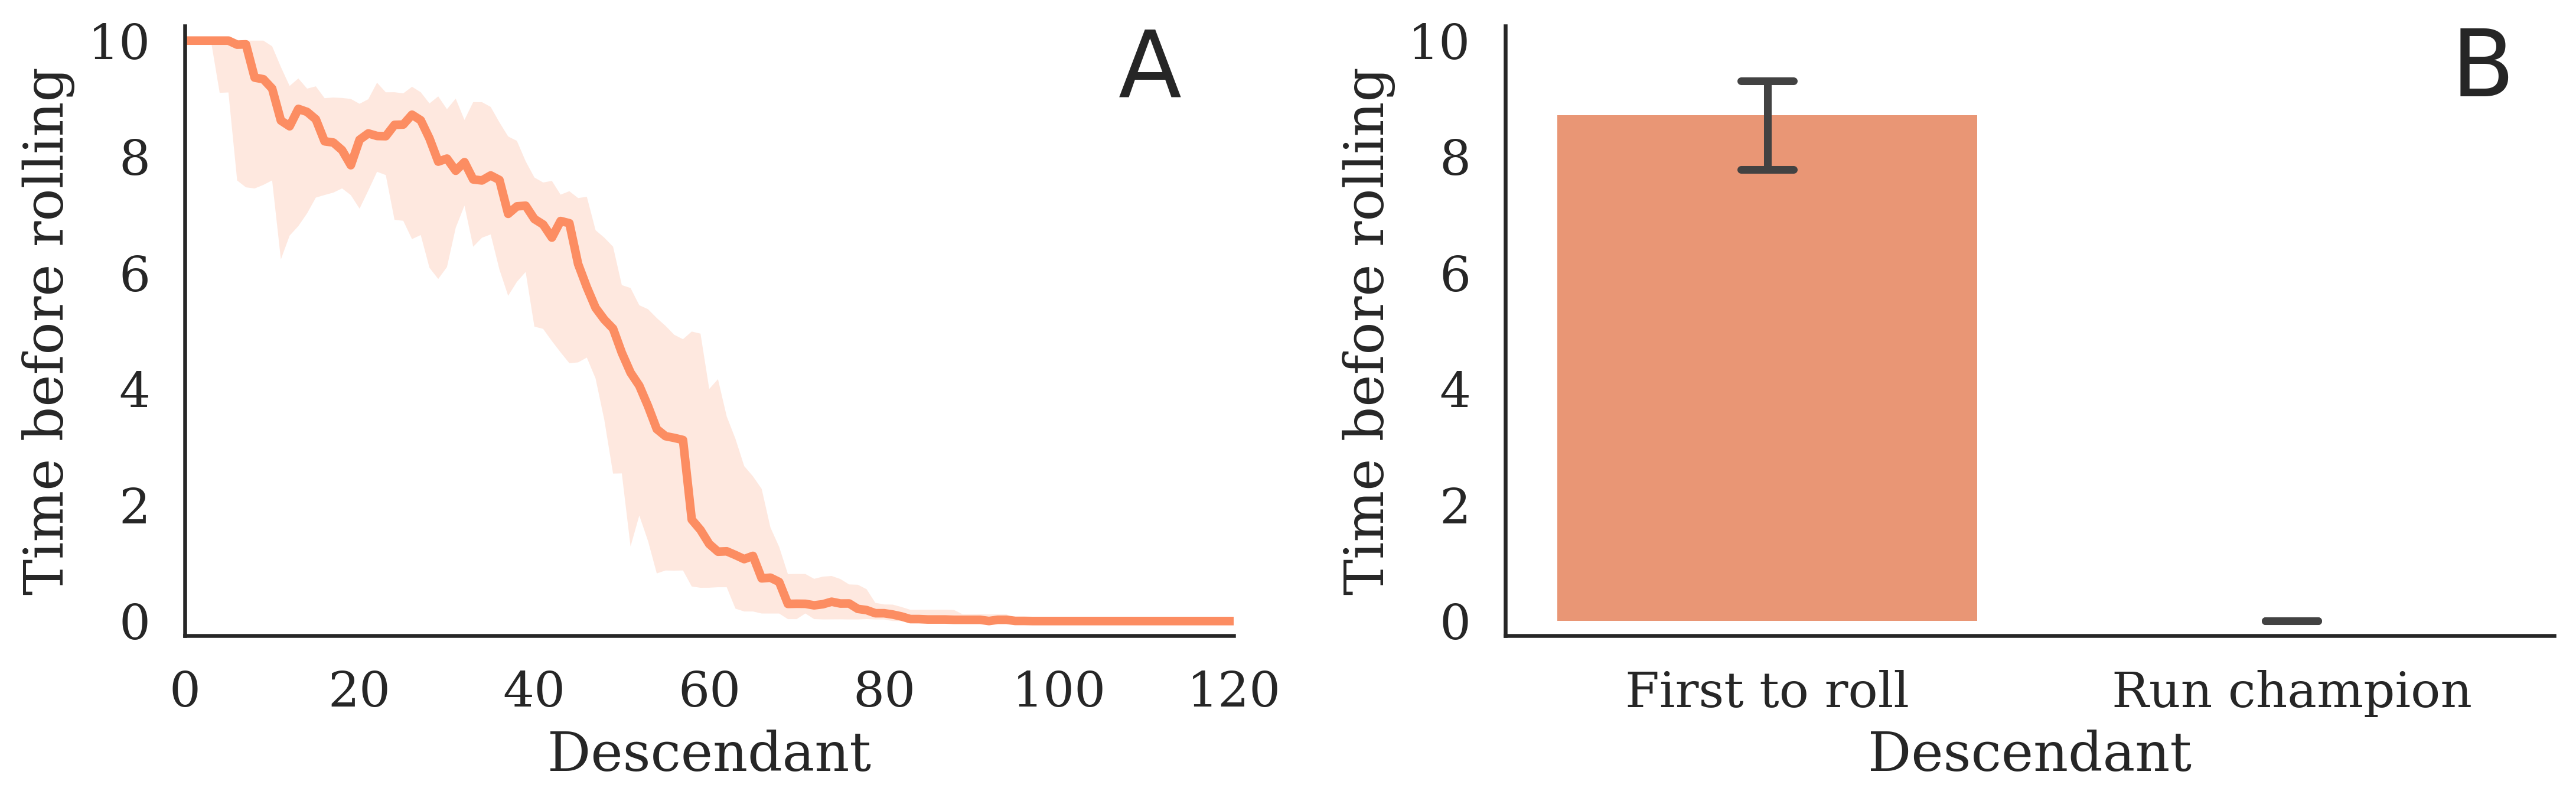
\includegraphics[width=0.9\linewidth]{Chapter04/Fig6}
\caption{\label{fig-discovery}\textbf{Late onset discoveries.} Ontogenetic time before the discovery of rolling over, taken from the lineages of the best robot from each of the 25 Evo-Devo trials that produced a rolling design. Median time to discovery, with 95\% C.I.s, for (A) the lineage from the most distant ancestor $(T=0)$ to more recent descendants, and (B) the first ancestor to roll over compared to the final run champion. 
Rolling over is measured from the first time step the top of the robot touches the ground, rather than after completely rolling over. 
The first ancestors to roll over tend to do so at the end of their lives, their descendants tend to roll sooner in life, and the final run champions all begin rolling immediately at birth. 
These results are a consequence of dependent time steps: 
because mutational changes affect all downstream steps, their phenotypic impact is amplified in all but the terminal stages of development. Thus, late onset changes can provide exploration in the search space without breaking rest-of-life functionality, and subsequent evolution can gradually assimilate this trait to the start of development.}
\end{figure}


\section{Results}
\label{sec4:results}

We consider a locomotion task, over flat terrain, for soft robots composed of a $4\times4\times3$ grid of voxels (Fig. \ref{fig:blueprint}).
Robots are evaluated for 40 actuation cycles at 4 Hz, yielding a lifetime of ten seconds. Fitness is taken to be distance traveled measured in undeformed body lengths (four unit voxels, i.e.~4 cm). 
Example robots are shown in Figures \ref{fig:blueprint} and \ref{fig:trot-gallop-roll}, and Supplementary \href{https://youtu.be/Ee2sU-AZWC4}{\color{blue}Video S1}.


All experiments were performed in the open-source soft-body physics simulator  
\textit{Voxelyze} \cite{hiller2014dynamic}. 
Voxelyze simulates soft materials using two elements: particles and beams. 
A particle is a point mass with rotational inertia.
% Two adjacent particles are connected by a spring-like beam, which has translational and rotational stiffness.
A spring-like beam (with translational and rotational stiffness) connects two adjacent particles.
Each particle is connected to at most six neighbors (above, below, front, back, left, and right), on a cartesian grid.
Local material properties are stored at particles and averaged across shared beams.
Finally, a voxel mesh is drawn around each particle for visualization, such that adjacent voxels touch at the center of their shared beam.
More details about how this is actually implemented are given by Hiller and Lipson \cite{hiller2014dynamic}.

The morphology of a robot is given by the resting (beam) length stored at each voxel (Fig. \ref{fig:blueprint}).
However the shape and volume of each voxel is changed by external forces from the environment and internal forces via behavior. 
The morphology of a robot is denoted by the $4\times4\times3=48$-element vector $\ell$, where each element is the resting length stored at that voxel (with possible values within $1.0 \pm 0.75\; \text{cm}$).
Like most animals, our robots are bilaterally symmetrical.
We built this constraint into our robots because bilateral symmetry is known to help with forward locomotion
\cite{grabowsky1994symmetry}.
The lefthand $2\times4\times3=24$ resting voxel lengths are reflected on the other, righthand side of the midsagittal line, yielding 24 independent resting lengths.

The controller, however, is not constrained to be symmetrical since many behaviors, even for symmetric morphologies, consist of asymmetric gaits, and is given by the phase offset of each voxel from a global oscillating signal with an amplitude of 0.14 cm. 
The controller is denoted by the 48-element vector $\phi$, where each element is the phase offset of that voxel (with possible values within $0 \pm \pi/2$). 


We investigated the impact of development in this model by comparing two experimental variants: Evo and Evo-Devo (schematized in Supplementary Fig. \ref{fig:S2}). % \hyperref[fig:S2]{S2}). 
The control treatment, \textbf{Evo}, lacks development and therefore maintains a fixed morphology and control policy in a robot as it behaves over its lifetime. 
Two parameters per voxel are sufficient to specify an evolved robot at any time $t$ in its lifetime: its morphology $\ell_k$, and controller $\phi_k$.
An evolutionary algorithm optimizes 24 morphological and 48 control parameters.

The experimental treatment \textbf{Evo-Devo} evolves a developmental program rather than a static phenotype (Fig. \ref{fig:blueprint}). 
For each parameter in an Evo robot, an Evo-Devo robot has two: its starting and final value.
The evolutionary algorithm associated with the Evo-Devo treatment thus optimizes 48 morphological and 96 control parameters.
The morphology and controller of the $k$-th voxel change linearly from starting to final values, throughout the lifetime of a developing robot.
The endpoint parameters are denoted by asterisks: the controller develops from $\phi$ to $\phi^*$, the morphology develops from $\ell$ to $\ell^*$.
The starting and final points of development are predetermined by a genome which in turn fixes the direction (compression or expansion) and rate of change for each voxel.
Development is thus \textit{ballistic} in nature rather than adaptive, as it cannot be influenced by the environment (Equation \ref{eq4:ballistic-devo}). 


For both treatments we conducted 30 independent evolutionary trials.
At the end of evolutionary optimization, the non-developmental robots (Evo) tend to move on average with a speed of 10 body lengths in 10 seconds, or 1 length/sec. The evolved and developing robots (Evo-Devo) tend to move at over 5 lengths/sec (Fig. \ref{fig-fitness}A).
To ensure evolved and developing robots are not exploiting some unfair advantage conferred by changing body plans and control policies unavailable to non-developmental robots, we manually remove their development by setting $\ell^*=\ell$ and $\phi^*=\phi$, which fixes the structure of their morphologies and controllers at birth ($t=0$) (Equation \ref{eq4:ballistic-devo}). 
That is to say, we convert the evolved Evo-Devo robots into Evo robots (Equation \ref{eq4:ballistic-devo} reduces to Equation \ref{eq4:no-devo}).
The resulting reduced robots suffer only a slight (and statistically non-significant) decrease in median speed and still tend to be almost five times faster than the systems evolved without development (Fig. \ref{fig-fitness}B, treatment `Evo-Devo removed').
Ballistic development is therefore beneficial for search but does not provide a behavioral advantage in this task environment.


To investigate this apparent search advantage, we trace development and fitness across the 30 lineages which produced a `run champion': the robot with highest fitness at the termination of a given evolutionary trial (Supplementary Fig. \ref{fig:S1}).% \hyperref[fig:S1]{S1}). 
We measure the amount of ballistic change in each robot|its `ballistic plasticity'|by a statistic we call the \textit{developmental window}.
The developmental window is defined separately for morphology (Equation \ref{eq-WL}) and control (Equation \ref{eq-WPhi}) as the absolute difference in starting and final values summed across the robot and divided by the total amount of possible development, such that 0 and 1 indicate no and maximal developmental change, respectively.
Evo robots by definition have development windows of zero, as do Evo-Devo robots that have had development manually removed.
An Evo-Devo robot with a small developmental window has thus become \textit{canalized} \cite{waddington1942canalization}.


In terms of fitness, there were two observed basins of attraction in average velocity: a slower design type which either trots or gallops at a speed of less than 1 length/sec (Fig. \ref{fig:trot-gallop-roll}A,B and Fig. \ref{fig-correlation}A{\Large$\ast$}), and a faster design type that rolls at 5-6 lengths/sec (Fig. \ref{fig:trot-gallop-roll}C). 
After ten thousand generations, 25 out of a total of 30 Evo-Devo trials (83.3\%) find the faster design, compared to just 6 out of 30 Evo trials (20\%).


\subsection*{Differential canalization.}

Modular systems are more evolvable than non-modular systems because they allow evolution to improve one subsystem without disrupting others \cite{wagner1996perspective,lipson2007principles}.
Modularity may be a property of the way a system is built, or it may be an evolved property.
The robots evolved here are by definition modular because the genes which affect morphology are independent of those which affect its control.
However the more successful Evo-Devo lineages evolved an additional form of modularity, which we term differential canalization:
Some initially developmentally plastic traits become integrated and canalized, while other traits remain plastic.


In the successful Evo-Devo trials, morphological traits were canalized while control traits were not.
Evidence for this is provided in Supplementary Fig. \ref{fig:S1},%\hyperref[fig:S1]{S1}, 
which is summarized by Fig. \ref{fig-correlation}A.
Trajectories of controller development (green curves) do not follow any discernible pattern in phylogenetic time, and appear upon visual inspection to be consistent with a random walk or genetic drift.
The trajectories of morphological development (red curves), however, follow a consistent pattern.
The magnitude of morphological development increases slightly, but significantly $(p<0.001)$, before decreasing all the way to the most recent descendant, which is the most fit robot from that trial (the run champion). 
Run champions tend to have much less morphological development than their most distant ancestor $(p<0.001)$, but there is not a significant difference between champion and ancestral controller windows.
Furthermore, this pattern tends to correlate with high fitness: in trials in which this pattern did not appear (runs 6, 8, 16-18), fitness did not increase appreciably over evolutionary time.

This process within the lineages of the run champions is consistent with a more general correlation found in all designs explored during optimization across all runs: Individuals with the highest fitness values tend to have very small amounts of morphological development, while their control policies are free to develop (Fig. \ref{fig-correlation}B).
However, despite the fact that morphological development tends to be canalized in the most fit individuals, it cannot simply be discarded as the non-developmental systems have by definition small morphological windows, and small controller windows, but also low fitness.  


To test the sensitivity of the evolved morphologies to changes in their control policies, we applied a random series of control mutations to the Evo and Evo-Devo run champions from each evolutionary trial.
For each run champion, we perform 1000 subsequent random controller mutations that build upon each other in series (a Brownian trajectory in the space of controllers)|and repeat this process ten times for each run champion, each with a unique random seed.
It was found that optimized Evo-Devo robots tend to possess body plans that are much more robust to control mutations than those of Evo robots (Fig. \ref{fig-random-walks}A).
The first control mutation to optimized Evo robots tends to immediately render them immobile, whereas optimized Evo-Devo robots tend to retain most of their functionality even after 1000 successive random changes to their controllers.
Within Evo-Devo designs, the functionality of the 25 fast designs are minimally affected by changes to their control, whereas the five slow designs also tend to break after the first control mutation (Fig. \ref{fig-random-walks}B). 
Thus it can be concluded that these five robots are non-modular: their non-canalized morphologies evolved a strong dependency on their controllers. 
The Evo robots are similarly non-modular: they are brittle to control mutations. 


To test the sensitivity of the evolved controllers to changes in their morphologies, we applied the same procedure described in the previous paragraph but with random morphological mutations rather than control mutations.
It was found that both developmental and non-developmental systems tend to evolve controllers that are very sensitive to morphological mutations (Fig. \ref{fig-random-walks}C).
These findings are consistent with those of Cheney \textit{et al.} \cite{cheney2018scalable}, who also reported that robots were more sensitive to changes in their morphology than in their controllers.
Here, the first few morphological mutations to optimized robots, in both treatments, tend to immediately render them immobile.
Within Evo-Devo design types, neither of which canalized development in their controllers (Supplementary Fig. \ref{fig:S1},% \hyperref[fig:S1]{S1}), 
both the fast and slow designs possess controllers sensitive to changes in their morphologies (Fig. \ref{fig-random-walks}D).
Thus it can be concluded that the non-canalized controllers evolved a strong dependency on their morphologies. 
Therefore the only trait to be successfully canalized was also the only trait that rendered the agent robust to changes in other traits.



\subsection*{Heterochrony in morphological development.}


The evolutionary algorithm can rapidly discover an actuation pattern that elicits a very small amount of forward movement in these soft robots regardless of the morphology. 
There is then an incremental path of increasing locomotion speed that natural selection can climb by gradually growing legs to reduce the surface area touching the floor and thus friction, and simultaneously refining controller actuation patterns to better match and exploit the morphology (Fig. \ref{fig:trot-gallop-roll}A,B).


There is, however, a vastly superior design partially hidden from natural selection---a `needle in the haystack', to use Hinton and Nowlan's metaphor \cite{hinton1987learning}.
On flat terrain, rolling can be much faster and more efficient than walking, but finding such a design is difficult because the fitness landscape is deceptive.
Rolling over once is much less likely to occur in a random individual than shuffling forwards slightly. And as a population continues to refine walking morphologies and gaits, lineages containing rocking individuals which are close to rolling over, or roll over just once, do not survive long enough to eventually produce a true rolling descendant. 

Development can alter the search space evolution operates in because individuals sweep over a continuum of phenotypes, with different velocities, rather than single static phenotype that travels at a constant speed (Supplementary Fig. \ref{fig:S2}E,J).% \hyperref[fig:S2]{S2}E,J).
The lineages which ultimately evolved the faster rolling design initially increased their morphological plasticity in phylogenetic time as evidenced by the initial upward trends in the red curves in Supplementary Fig. \ref{fig:S1}% \hyperref[fig:S1]{S1} 
(summarized by Fig. \ref{fig-correlation}A) which contain a statistically significant difference between their starting and maximum developmental window sizes $(p<0.001)$.
This exposes evolution to a wider range of body plans and thus increases the chance of randomly rolling at least once at some point during the evaluation period.

The peak of morphological plasticity in  Supplementary Fig. \ref{fig:S1}% \hyperref[fig:S1]{S1}
(summarized by Fig. \ref{fig-correlation}A) generally lines up with the start of an increasing trend in fitness (blue curves) and marks the onset of differential canalization.
Rolling just once allows an individual to move further (1 body length) than some early walking behaviors but they incur the fitness penalty of having fallen over and thus not being able to subsequently walk for the rest of the trial. 
Therefore this tends to happen at the very end of ontogeny (Fig. \ref{fig-discovery}), as individuals evolve to `dive' in the last few time steps of the simulation of their behavior, thus incurring an additional increase of fitness over their parent, which does not exhibit this behavior.
Since more rolling incurs more fitness than less rolling, a form of progenesis occurs as heterochronic mutations move $\ell_k$ closer to $\ell_k^*$, for each voxel.
This gradually earlifies rolling from a late onset behavior to one that arises increasing earlier in ontogeny (Supplementary \href{https://youtu.be/Ee2sU-AZWC4}{\color{blue}Video S1}).
As more individuals in the population discover and earlify this rolling behavior, the competition stiffens until eventually individuals which are not born rolling from the start are not fast enough to compete (Fig. \ref{fig:trot-gallop-roll}C,D).


\subsection*{Generality of results.}


For the results above, as in nature \cite{lynch2010evolution}, the mutation rate of each voxel was left under evolutionary control (self-adaptation).
In an effort to assess the generality of our results, we replicated the experiment described above for various fixed mutation rates (Supplementary Fig. \ref{fig:S3}).% \hyperref[fig:S3]{S3}).
Without development, as in Hinton and Nowlan's case\cite{hinton1987learning}, the search space has a single spike of high fitness. 
One can not do better than random search in such a space.
At the highest mutation rate, optimizing Evo morphologies reduces to random search, and this is the only mutation rate where Evo does not require significantly more generations than Evo-Devo to find the faster design. 
This can be observed in Supplementary Fig. \ref{fig:S3}  % \hyperref[fig:S3]{S3} 
by comparing the generation at which the slopes of the fitness curves increase dramatically. 
However, the best two treatments, as measured by the highest median speed at the end of optimization, have development, and the robots they produced are significantly faster than those produced by random search (Evo with the highest mutation rate) $(p<0.01)$.

To further test the sensitivity of our results to the various settings of our particular system,
we transcribed the main experiment for a different class of morphologies (rigid bodies) and controllers (neural networks).
Details are provided in Supplementary Fig. \ref{fig:S5} %\hyperref[fig:S5]{S5} 
and Supplementary Methods.
The results of this test indicate that differential canalization exists elsewhere, but it does not always increase evolvability.  


